%%%%%%%%%%%%% 5 %%%%%%%%%%%%%%%%%%%%%%%%%%%%%%%%%%%%%%%%%%%%%%%%%%%%%%%%%%%%%%%%%%%%%%%%%%%%%%%%%%%%%%%%%%%%%%%%%%%%%%%%
\chapter{Cosmic Ray Search with ANITA3 Flight Data}
%%%%%%%%%%%%%%%%%%%%%%%%%%%%%%%%%%%%%%%%%%%%%%%%%%%%%%%%%%%%%%%%%%%%%%%%%%%%%%%%%%%%%%%%%%%%%%%%%%%%%%%%%%%%%%%%%%%%%%%%
\section{ANITA3 Flight Overview}
	The data recorded by the ANITA3 flight instrument requires a significant analysis effort to extract a meaningful physics result.  In our case, we need to use the raw digital values read out for each channel to determine the analog electromagnetic environment surrounding the payload during brief moments the trigger system determined a physics event may be occurring.  From this, we can use an understanding of the physical geometry of the antennas mounted on the payload, including their orientation and electrical responses, to determine the cause of any incident wave patterns read out by the digitizers.  Once these wave patterns are identified and classified, they can be sorted into signal and noise, background thermal or anthropogenic, via a series of procedural cuts.  This section details the process and results of this analysis.
	
\section{Analysis Overview}
	The analysis for this flight was done with the premise that we are searching for "cosmic ray like" events.  As there are already published observations of cosmic rays from previous ANITA flights, I can reduce the workload of doing a full blind analysis with the consequence of excluding signals that do not fit into a measured and modeled EAS radiation pattern.  This still will allow us to search for two separate cosmogenic particles, cosmic rays and tau neutrino regeneration events.

	\subsection{In Flight Modifications}
		The majority of the ANITA3 flight required very little input from ground operators.  However there were some minor issues in the beginning of the flight that required fixing, and one in the middle of the flight that resulted in lost data.
		
		At the beginning of the flight, the default time persistance values for phi masking were set too high, resulting in the entire payload becoming masked as it rotated.  The solution to this was to lower the values so that phi masking was turned off as scalar rates dropped back to manageable levels.
		
		Between run s
	
\section{Blinding Procedure}
	Avoiding the introduction of bias into the resulting measurement through the subconsious desires of the analyzer is a constant struggle.  Several techniques have been employed to minimize this insidious bias.
	
	\subsection{Philosophical Reasoning For Blinding}
		
	\subsection{Threshold for Unblinding Request}
		
	\subsection{Polarization Specific Blinding}

\section{Event Quality Cuts}
	Events taken with the ANITA instrument must first pass basic checks on their quality.  


\section{Constant wave source filtering}
	Anthropogenic signals used for communications often take the form of high powered circularly polarized constant wave sources.  These signals are present in much of the data, and their effect on the trigger is twofold.  Firstly, they compress the tunnel diode by increasing the total power of the input signal, elevating the diode response out of the square-law range.  Second, they force an increase in the threshold voltage used on the comparator circuit used to trigger on the signals.  Despite these two effects, impulsive candidate signals can still be hidden superimposed on the CW source.  To remediate the effects of these signals on the pointing and post-flight analysis, we can apply a filter that only notches out a specific frequency band of the signal.
	\subsection{Bookkeeping and Filtering Decision Heuristic}
	\subsection{Fourier Domain Band Filtering}
			The easiest way to filter out CW signals is to set the magnitude of the complex Fourier phasors to zero in frequency bands that exceed some expected flat spectral slope.  Though this is computationally quite easy, this process is not causal, and will harm the integrity of the resultant signal.
		\subsection{Sine wave subtraction}
			A more computationally intensive method for eliminating CW sources is a method where a sine wave is fit to the measured waveform and iteratively subtracted.  This process preserves the causality of the signal, as it is done purely in the time domain, and also decreases the width of the band that will be filtered, preserving more total signal power if it exists in the measurement.  The drawback of this method is that it requires a fit, which is takes time and is prone to failure.


\section{De-dispersion}
	The antenna, filters, cables, and amplifiers are responsible for introducing a frequency dependent gain and group delay to the observed signals.  These elements act to disperse the power in the signal across tens of nanoseconds from what was emitted from the relativistic shower at the critical angle as a highly impulsive, picosecond length essential delta-function like electromagnetic field transient.  The impulse response, or complex phasor representation of this dispersive effect, was measured for the signal chain immediately preceding the flight for each of the 96 channels, and for all 48 antennas in a controlled manner in Palestine the summer beforehand.  These two effects are then combined and used to determine a whole system impulse response that relates the measured ADC values at the LABRADOR digitizer to an electric field incident at the payload.  By reversing the dispersive process, via Weiner deconvolution (described below), we can both increase the instantaneous power of a signal and compare it directly to the electric field radiation output of high energy particle shower simulations such as COREAS or ZHAires.
	\subsection{Generation of transfer function}
		The transfer function of the system was painstakingly developed and utilized a variety of both time domain and Fourier transformed frequency domain manipulations.  These each introduce their own errors, as many of them require assumptions about the incoming signal.  I'll detail the full process of generating the transfer function in an appendix.
	\subsection{Signal to noise ratio of impulse response}
		Any band limited deconvolution process requires a knowledge of the signal to noise ratio of the transfer function as a function of frequency (SNR(f)).  Since the transfer function merely relays the amplitude and phase differences between an input and output signal (represented in either a complex phasor or a time domain waveform), one must also have an understanding of the total power contained within the input and output signals.  If, for example, both the input and output signal contained very little power out of a specified band pass, it could be wrongly assumed from a transfer function that the signal chain was able to pass frequencies that are out of the band pass.
		The "signal" and "noise" of this must therefore be defined, as the spectral power has multiple sources.  The principle   
	\subsection{All-Pass Deconvolution}
		The impulse response used to deconvolve waveforms has been colloquially named the All-Pass deconvolution method.  An ideal deconvolution, one that uses both phase and amplitude information to remove the instrument response, is poorly defined outside the instrument bandwidth.  Since the instrument blocks any signal outside this frequency range, reversing the procedure introduces what is in essence a "divide by zero" error that grossly amplifies signal power outside the band.  The simplest way to avoid this is to disgard the frequency dependent amplitude information, and only correct for the phase.  Due to the relatively flat spectral response of the ANITA system, this is a good first approximation.  The resulting waveform "stacks" signal power from all in-band frequencies on top of one another, increasing the observed peak to peak signal to noise ratio and offering a larger separation between signal and noise events during analysis cuts.

\section{Polarization cuts}
	The expected signal from a cosmic ray air shower has a characteristic polarization that can be used as a further discriminator between random noise, which will have a random polarization.  Specifically, the geomagnetically induced radiation component will be linearly polarized and orthogonal to both the shower axis and the magnetic field.  This allows two cuts to be made, one of the linear polarization fraction and one of the linear polarization angle.  Both these rely on the calculation of Stokes parameters made possible by the dual polarization antennas, which capture both these time domain electric fields simultaneously.

	\subsection{Linear Polarization Fraction}
		
	\subsection{Linear Polarization Angle}

	
\section{Event Reconstruction}
	The major tool used in the ANITA analysis is interferometry, a radio astronomy technique that uses the physical separation between the antennas and the correlations of waveforms from these antennas to generate a map of likely pointing directions.  ANITA has three vertical tiers of antennas, each separated from each other, and at least three co-pointing phi sectors that are expected to observe events from any angle.  Using the combined baseline offsets from these antennas, it is possible to overlay 9 different interferometric maps to create a pointing map.  By finding the peak of this map, a vector pointing away from the payload can be traced to the ice, where a map of the vertical height of the continent can be used to create a map of events on the ground.
	
	\subsection{Radio Interferometric Mapping}
		Interferometric mapping is a method developed to compare measured time domain waveforms captured by antennas with a physical baseline offset with the goal of determining likely incoming plane wave direction.  This is accomplished by calculating the timing offsets expected from each direction of a pair of antennas in elevation and azimuth, computing the correlation function of the two waveforms, then weighting each direction in relation to the correlation value at that specific timing offset.  An example of a map created with a single baseline pair is seen in Figure \ref{fig:singleBaselineCorrMap}.  With multiple baseline pairs, each with a different distance vector angle between them, one can overlay multiple correlation maps to determine a most likely incoming plane wave direction.
		
		
	\subsection{Coherent Sum Averaging}
		The electronic and thermal noise present in each channel limits the sensitivity of the instrument to EAS signals with low power.  Since the power within the radiation of an EAS shower varies linearly with the energy of the particle, low energy showers, which have a higher flux rate, will have signal to noise ratios approaching one.  Additionally, polarization information and frequency content are effected by any noise present in the system.  Averaging waveforms from multiple channels will reduce this incoherent background noise by a factor of $\frac{1}{\sqrt{N}}$.  After determining the peak interferometric pointing direction, it is possible to align the channels that received signal from an incident radiation field and average them together.  An example of this is shown in Figure \ref{fig:coherentSum}.
	
	
	\subsection{Ray Tracing to Continent (with index of refraction)}
		Another tool made possible through interferometric mapping is that it allows us to point a captured event back to its incoming direction, determining the likely incident cosmic ray interaction location.  Ultimately, it would be most interesting to point an incoming particle back to a location on the sky for statistical source determination.  Additionally, it is important to determine whether a measured event came from a particle physics interaction, or was merely an anthropogenic background noise impulse.  By developing a base list from USAP and other international Antarctic programs, we can determine whether a specific event points back to a known base.

	
	\subsection{Immediate Pointing Cuts}
		Real physics signals have a small range of elevation angles where their detection is most likely.  The highest probability incident direction for an EAS is near the horizon, however noise events will point more evenly in all directions.  Using this knowledge, we can cut out events that have very steep elevations.  A distribution of event pointing direction can be seen in Figure \ref{fig:elevationAngle}.

\section{Template Correlation}
	Though any physics experiment that aims to separate background events from signal events requires a general understanding of characteristics inherent to either group, measurements and simulations of UHECR induced EAS signatures provide a waveform template that can be used to strongly cut on signal events.  The simplest assumption, that an EAS will produce a broad spectrum, short duration, electromagnetic pulse, drives both the overall design of the payload, as well as several of the analysis cuts.  Determining a normalized correlation between a template and the coherently summed waveform provides an additional constraint beyond simply requiring impulsivity, and also requires the gain and phase characteristics of an incident wave are in agreement with an EAS signal.
	
	\subsection{Templates}
		It is possible to generate several different templates that accurately represent an observable EAS signal on the payload.
	
	\subsection{Auto-correlation normalization}
		In order to make the template correlation value of different events directly relatable to one another, it is important to normalize both the template and the coherently summed waveform.  As this measurement is most interesting in determining the amount that any given event ``looks'' like the template, the final value should be a fraction from 0 to 1, where 1 would be a waveform that is an exact copy of the template.  


\section{Known object categorization}
	Many bases on the Antarctic continent are already cataloged by the various national programs that operate them.  Using these known bases we can eliminate events that interferometrically point to objects of expected anthropogenic noise.  There also likely exist bases that are, for whatever reason, not included in our catalog.  We also use a list of "pseudo-bases" generated from clustered event lists from previous ANITA flights to eliminate possible anthropogenic interference.  The resulting effect these excluded regions have on the flight can be determined by its flight path and a log-likelyhood method for generating pointing error elipses around the bases.  I'll put a plot of that here.
	\subsection{Sun and Its Reflection, Thermal Noise Effect}
	\subsection{Satellites, Bases, and other Anthropogenic Sources}

\section{Thermal Noise Separation Results}
	\subsection{Cut Efficiency}
	\subsection{Cut Quality}




\section{Base and event clustering}
	
	After enriching the event sample by removing events with a high probability of being thermal noise or non-impulsive anthropogenic background, geographical clustering of the events can be done to further discriminate against backgrounds. Physics signal events are expected to be isotropically distributed evenly across the continent, as there is no preferred cardinal direction for UHECR or UHE$\nu$ detections.  Human activity, on the other hand, tends to cluster around regions of logistical or scientific interest.  Anthropogenic background sources are thus expected to point at other captured events, which can be used to discriminate against them and further refine the data sample. 

	\subsection{Base Clustering}
		Through communication with various Antarctic institutions, a list of active camps and other human activity on the continent was compiled for the time frame of the ANITAIII flight.  An image of these bases mapped to the continent can be seen in Figure \ref{fig:BaseMap}.  Determining the validity of this base map is plagued with issues, as they are run an managed by a large collection of different nations and groups, many of whom do not wish or care to make their activities publicly available.  Additionally, camps that are reported by groups may be inactive, or have moved from when they were last reported.  Despite these limitations, it is still useful to map events that pass signal cuts to these bases.
		
\begin{figure}
	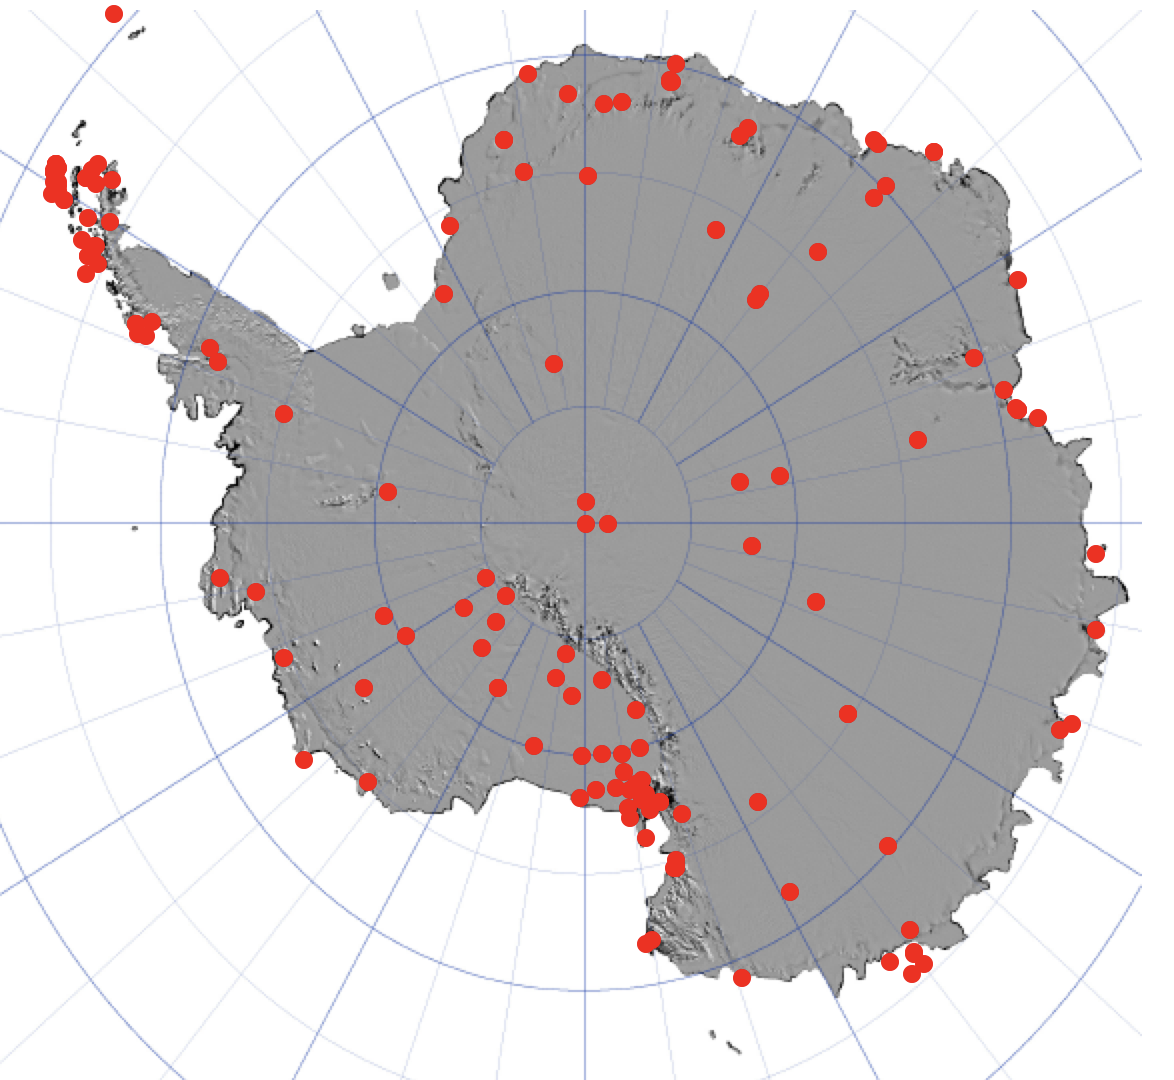
\includegraphics[width=\textwidth]{figures/BaseMap}
	\caption{A map of the recorded human activity on the continent of Antarctica during the ANITAIII flight.}
	\label{fig:BaseMap}
\end{figure}	
	
	
	\subsection{Event Clustering and Log Likelihood}
		The metric that has been used in past ANITA experiments to determine the ``closeness'' of one event to another has been called the Log Likelihood, and is represented by the variable $L$.  This measurement must take into account both the pointing uncertainty of the instrument, as well as the constantly changing payload location.
		
		The pointing resolution of the interferometric mapping technique is a function of the SNR, and thus any clustering analysis must factor this into its calculation.  The pointing resolution as a function of SNR was found from analyzing self triggered WAIS pulses and their subsequent pointing to the 
		
		As ANITA transits past anthropogenic sources on the continent, the payload coordinate pointing towards that base changes with respect to cardinal North. In order to determine whether the likelihood that any particular event fell close to another, one must project the geographical location where the first event pointed to the continent into the field of view of the second event payload locations.  The opposite must be done as well, projecting the second event source location into the field of view of the first event payload location, as the two processes are not strictly invertible.
	\begin{equation}
		L = \sqrt{(\frac{\sqrt{(\Delta\phi_{AB})^2+(\Delta\phi_{BA})^2}}{{\sigma_{\phi}}})^2+(\frac{\sqrt{(\Delta\theta_{AB})^2+(\Delta\theta_{BA})^2}}{{\sigma_{\theta}}})^2}
	\end{equation}
	
